\documentclass[tikz,border=1.35mm]{standalone}

\definecolor{fvmadaptedge}{HTML}{8A7E7E}

% Plain triangular face used in the FVMAdapt overview figures.
% Coordinates are in millimeters; y=-1mm keeps the SVG-style origin at top left.
\begin{document}
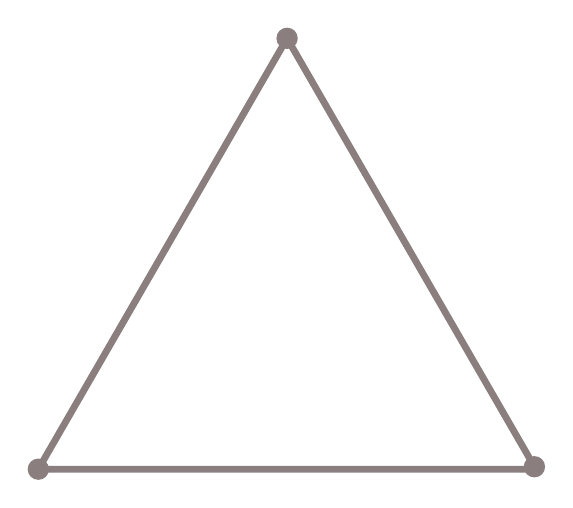
\begin{tikzpicture}[x=1mm,y=-1mm,line join=round]
  % Match the original artwork frame before the standalone border is applied.
  \useasboundingbox (0,0) rectangle (65.711,57.425);

  % Triangle vertices.
  \coordinate (v0) at (1.353,56.073);
  \coordinate (v1) at (64.538,56.073);
  \coordinate (v2) at (32.945,1.353);

  % Draw edges first so vertex markers sit cleanly on top.
  \draw[draw=fvmadaptedge,line width=0.865mm] (v1) -- (v0) -- (v2) -- cycle;

  % Original vertices are #8a7e7e.
  \fill[fvmadaptedge] (32.945,1.353) circle[radius=1.353mm];
  \fill[fvmadaptedge] (64.358,55.762) circle[radius=1.353mm];
  \fill[fvmadaptedge] (1.353,56.073) circle[radius=1.353mm];
\end{tikzpicture}
\end{document}
